All models used Adam with learning rate $10^{-3}$, weight decay $10^{-4}$, batch size 32, dropout 0.3, cosine annealing over at most 80 epochs, gradient clipping at 1.0, and early stopping with patience 10 on validation macro-F1. Experiments used seeds 42, 43, and 44, deterministic execution, and \texttt{num\_workers=0}. The environment was WSL2 Linux with Python 3.11.15, PyTorch 2.0.0+cu117, NumPy 1.26.2, cuDNN 8.5.0, and an RTX 3050 Laptop GPU.

\subsection{Held-Out-Performer Evaluation}

For each eligible target performer, every sample from that performer forms the test fold, and training and validation draw only on the others:
\begin{equation}
\mathcal{P}_{\mathrm{train}}\cap\mathcal{P}_{\mathrm{test}}
=
\mathcal{P}_{\mathrm{val}}\cap\mathcal{P}_{\mathrm{test}}
=
\varnothing.
\label{eq:performer_disjoint}
\end{equation}
Note that Eq.~\eqref{eq:performer_disjoint} constrains performer sets, not sample sets; this is the distinction the rest of the paper turns on. Hòa Đê yields $5\times4\times3=60$ runs and fingerspelling $5\times2\times3=30$. We average performer-level results over the three seeds, then average across eligible performers to obtain an architecture mean. Performers are the independent evaluation units, not samples and not seeds.

\subsection{Matched Performer-Exposure Experiment}

To isolate what performer exposure alone is worth, we hold the test set still and vary only what development sees (Fig.~\ref{fig:matched_protocol}). For each Hòa Đê performer, roughly half the samples form a fixed, class-balanced test set; the remainder become an exposure pool. Protocol A keeps the target performer out of training and validation. Protocol B moves disjoint exposure-pool samples into both development partitions, leaving the fixed test sample identifiers untouched:
\begin{equation}
\mathcal{T}_p\cap
\left(
\mathcal{D}^{B}_{\mathrm{train}}\cup
\mathcal{D}^{B}_{\mathrm{val}}
\right)=\varnothing.
\label{eq:test_disjoint}
\end{equation}
Matching matters here, so the added target-performer training samples displace class-matched samples from other performers. Training size and per-class training counts therefore stay fixed across the two protocols. Only validation composition changes, and it changes deliberately, because checkpoint selection is half of what we are measuring.

For model $m$ and performer $p$, the exposure gap is the difference between the two accuracies on that same fixed test set:
\begin{equation}
\Delta_{m,p}=a^B_{m,p}-a^A_{m,p}.
\label{eq:exposure_gap}
\end{equation}
The experiment comprises $5\times4\times2\times3=120$ valid runs. One caveat travels with Eq.~\eqref{eq:exposure_gap}: because early session provenance is incomplete, $\Delta_{m,p}$ may absorb session-related similarity alongside performer-related similarity.

\begin{figure}[tbp]
\centering
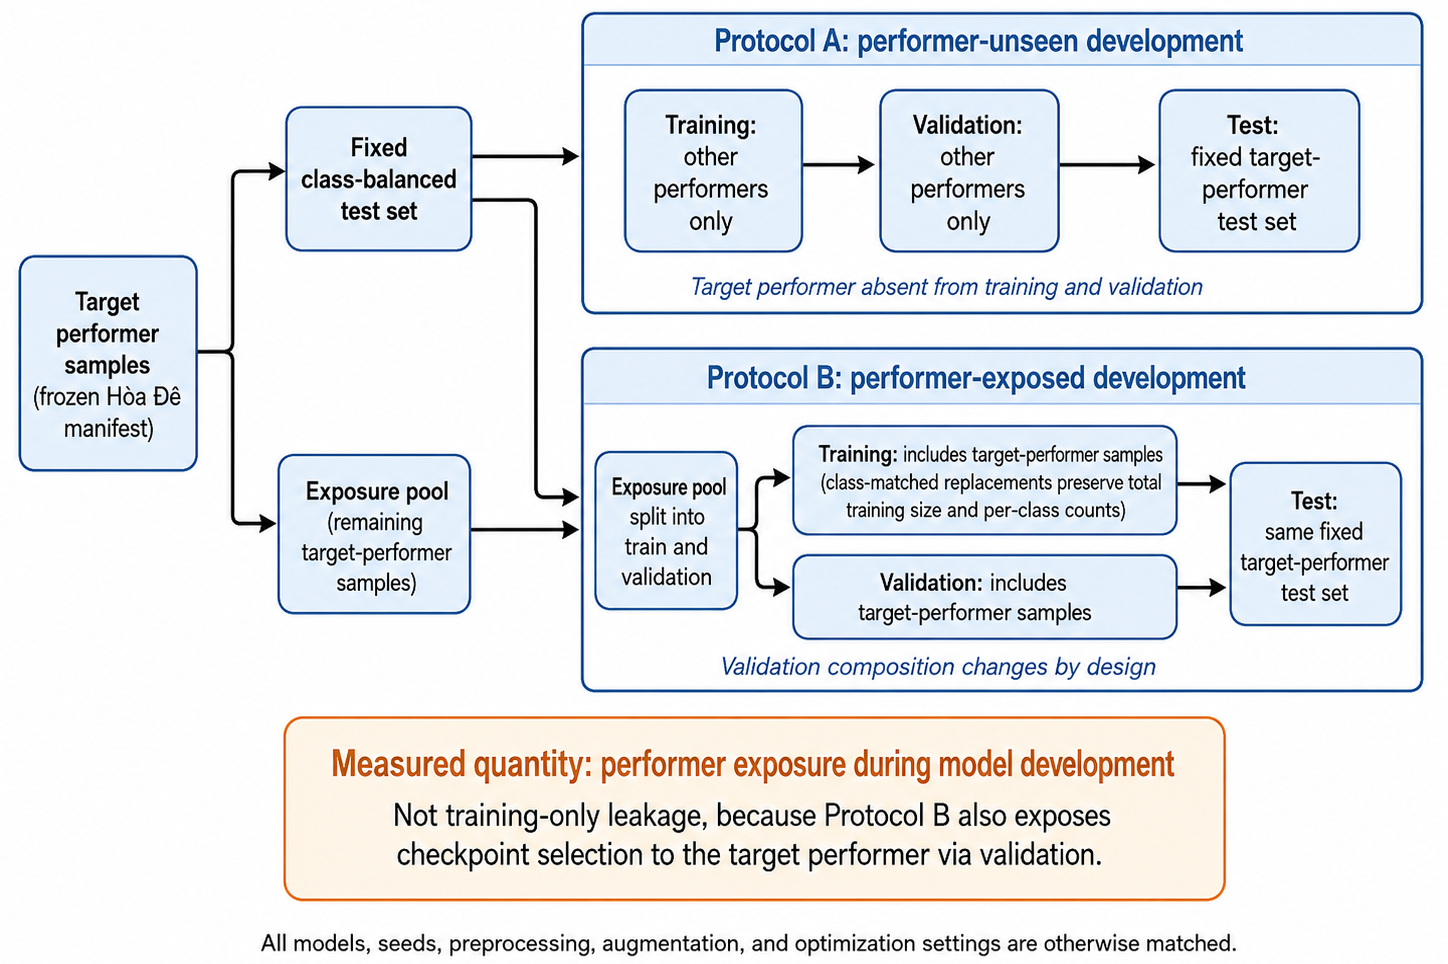
\includegraphics[width=0.90\linewidth]{Figures/Figure2_matched_protocol.png}
\caption{Matched performer-exposure protocol. Both conditions use the same fixed target-performer test set; Protocol A excludes the target performer from training and validation, while Protocol B introduces disjoint target-performer samples into both development partitions.}
\label{fig:matched_protocol}
\end{figure}

\subsection{Models, Baselines, and Metrics}

\begin{table}[htbp]
\centering
\caption{Evaluated neural architectures.}
\label{tab:models}
\small
\setlength{\tabcolsep}{4pt}
\renewcommand{\arraystretch}{1.1}
\begin{tabularx}{\linewidth}{l L r}
\toprule
\textbf{Model} & \textbf{Core configuration} & \textbf{Parameters} \\
\midrule
HandGCN & 42-node hand graph; two distance-aware GCN layers; part pooling; temporal attention & 135,711 \\
TCN & Three dilated temporal blocks; 64 channels; temporal attention & 133,960 \\
CNN & Three temporal convolutions; max pooling; global average pooling & 281,162 \\
LSTM & Two bidirectional layers; hidden size 64; global average pooling & 206,343 \\
BiGRU+Attn & Two bidirectional GRU layers; hidden size 64; self-attention & 206,471 \\
\bottomrule
\end{tabularx}
\end{table}

Table~\ref{tab:models} lists the five architectures and their parameter counts. Alongside them we evaluated uniform-chance, majority-class, Euclidean nearest-centroid, and Euclidean 1-NN baselines on flattened $60\times126$ sequences, keeping the zero-valued missing-hand slots so that the baselines see exactly what the networks see. Accuracy and macro-F1 were recorded for every run, and validation macro-F1 selected the checkpoint. With four performers as our independent units, we keep the analysis descriptive and report no sample-level significance tests.

\subsection{Reproducibility Protocols}

Our same-code test repeated two executions of commit \texttt{28f0393} for HandGCN, CNN, and TCN, holding the RTX 3050 environment, seed, split, and 80-epoch configuration constant, and compared model-state tensors, predictions, metrics, and metadata exactly. A second test compared 90 corresponding configurations across commits \texttt{0475b78} and \texttt{7ee3fbd}. Since the source revisions differ there, we read that result as optimization robustness and not as determinism.